\section{Use Cases of Hubble}
\label{sec:use_cases}

\begin{table}[tb]
\centering
\small
\caption{\textbf{ROC AUC scores of baseline MIAs for our largest perturbed model (8B, 500B tokens).} \textit{Dup} indicates the duplication level of members. \textit{Dup $\neq$ 0} treats all inserted perturbations as members. Non-members are always drawn from perturbations inserted 0 times. As duplication increases, memorization becomes stronger, and it becomes easier for membership inference attacks (MIA) to distinguish between members and non-members. See Appendix \ref{app:mia_results} for more \textsc{HubbleMIA} settings.}
\label{tab:hubble_mia_8b_perturbed}
\begin{tabular}{clcccccc}
\toprule
\multirow{2}{*}{\textbf{Evaluation}} & \multicolumn{1}{c}{\multirow{2}{*}{\textbf{MIA}}} & \multicolumn{6}{c}{\textbf{\textsc{Hubble} 8B (500B tokens) Perturbed}}                         \\ \cmidrule(lr){3-8} 
                                     & \multicolumn{1}{c}{}                                        & Dup $\neq$ 0 & Dup = 1 & Dup = 4 & Dup = 16 & Dup = 64 & Dup = 256 \\ \midrule
\multirow{4}{*}{\shortstack{Gutenberg\\Unpopular}} & Loss                                                        &   0.629       &   0.539      &  0.556       &   0.732       &   \textbf{0.996}       &  \textbf{1.0}           \\  
                                     & MinK\%                                                      &   0.629       &   0.539      &  0.556       &   0.732       &   \textbf{0.996}       &  \textbf{1.0}           \\  
                                     & MinK\%++                                                    &   \textbf{0.666}       &   \textbf{0.545}      &  \textbf{0.62}       &   \textbf{0.813}       &   0.987       &  0.949           \\  
                                     & ZLib                                                        &   0.622       &   0.53      &  0.551       &   0.722       &   \textbf{0.996}       &  \textbf{1.0}           \\
\midrule
\multirow{4}{*}{\shortstack{Yago\\Biographies}}    & Loss                                                        &   0.692       &   0.538      &  0.652       &   \textbf{0.897}       &   \textbf{1.0}       &  \textbf{1.0}           \\  
                                    & MinK\%                                                      &   0.692       &   0.537      &  0.651       &   0.896       &   \textbf{1.0}       &  \textbf{1.0}           \\  
                                    & MinK\%++                                                    &   \textbf{0.714}       &   \textbf{0.571}      &  \textbf{0.686}       &   0.892       &   0.995       &  0.983           \\  
                                    & ZLib                                                        &   0.676       &   0.524      &  0.633       &   0.872       &   \textbf{1.0}       &  \textbf{1.0}           \\
\midrule
\multirow{4}{*}{MMLU}                & Loss                                                        &   0.673       &   0.529      &  0.628       &   0.857       &   \textbf{1.0}       &  \textbf{1.0}           \\  
                                    & MinK\%                                                      &   0.672       &   0.529      &  0.626       &   0.854       &   \textbf{1.0}       &  \textbf{1.0}           \\  
                                    & MinK\%++                                                    &   \textbf{0.743}       &   \textbf{0.58}      &  \textbf{0.731}       &   \textbf{0.943}       &   0.994       &  0.986           \\  
                                    & ZLib                                                        &   0.644       &   0.523      &  0.593       &   0.775       &   0.993       &  0.999           \\
\bottomrule
\end{tabular}
\end{table}


The randomized perturbations in \textsc{Hubble} are designed to enable a broad range of research on LLM memorization. To demonstrate this, we establish new benchmarks for both membership inference attacks (MIAs) and unlearning. Membership inference is the task of inferring which data was part of a  model's training set and MIAs are used to audit privacy risks of trained models  \citep{shokri2017membershipinferenceattacksmachine}. Machine unlearning erases  harmful knowledge or behaviors from models while preserving other capabilities, without requiring full retraining \citep{bourtoule_2021_machine, llm_unlearning}.

\subsection{Hubble as an MIA Benchmark}
\label{sec:hubble_as_mia}

\textbf{Current MIA benchmarks for LLMs.}~ \citet{minkMIA} introduces \textsc{WikiMIA}, a membership inference benchmark for LLM pretraining data. \textsc{WikiMIA} labels Wikipedia articles before and after a model’s knowledge cutoff as members and non-members, respectively. However, subsequent analyses found that spurious features (such as temporal cues) allow non-members articles to be trivially distinguished from members, undermining the benchmark's validity \citep{duan2024membershipinferenceattackswork,meeus_sok_2025, naseh2025syntheticdatamisleadevaluations}. At the same time, this line of work shows that detecting pretraining data is generally difficult. When using the randomized train and test sets of Pythia, most membership inference methods achieve only marginal performance.

\textbf{The \textsc{HubbleMIA} benchmark.}~\textsc{Hubble} provides a sound benchmark for evaluating membership inference on several data types, including book passages, PII, and standard evaluation test sets. Since each perturbation is randomly duplicated zero or more times, there are no spurious features that inadvertently leak membership information. Perturbations in \textsc{Hubble} are also decontaminated and inserted at different frequencies, allowing comparisons of membership inference effectiveness on low- versus highly-duplicated examples. % Evaluating MIAs on the standard models (which were not trained on the perturbation data at all) serves as a sanity check, and when AUC is different from 50\%, MIA methods incorrectly detect non-members as members (false positive) at a rate higher than random chance.

\textbf{Experimental setup.} We instantiate 12 membership inference settings as a representative subset of all possible MIA benchmarks enabled by the Hubble Suite: 4 Hubble model variants (two perturbed models and two standard models) on 3 perturbation datasets each (Gutenberg Unpopular, YAGO Biographies, and MMLU). MIAs are evaluated with perturbations duplicated zero times as non-members, and perturbations duplicated more than once as members. For this evaluation, we employ off-the-shelf implementations from OpenUnlearning \citep{dorna2025openunlearningacceleratingllmunlearning}, specifically testing Loss-based \citep{LossMIA}, MinK\% \citep{minkMIA}, MinK\%++ \citep{minkplusplusMIA}, and Zlib-based attacks \citep{carlini_extracting_2021}.

\textbf{Results.} Table~\ref{tab:hubble_mia_8b_perturbed} reports MIA performance of Gutenberg Unpopular for our most capable model (8B, 500B tokens). MIA performance on all datasets and models are presented in Appendix~\ref{app:mia_results}. Across all benchmarks, membership inference performance consistently improves as the duplicate count increases, and attacks are strongest when distinguishing non-members from members duplicated 256 times.  However, distinguishing members duplicated only once produces near-random results, which confirm observations in \citet{duan2024membershipinferenceattackswork} that MIAs perform well only on members that are highly duplicated. Generally, our results show MinK\%++ to be the most effective attack. Surprisingly, MinK\%++ does not achieve 100\% AUC on the highly duplicated samples, unlike simpler approaches such as Loss and MinK\%.

\subsection{\textsc{Hubble} as an Unlearning Benchmark}

\textbf{Current LLM unlearning benchmarks.} Existing benchmarks target different aspects of machine unlearning. TOFU \citep{tofu} focuses on the unlearning of private data through  synthetic biographies. However, TOFU operates in a fine-tuning setting, where models are fine-tuned on the data to be forgotten. MUSE \citep{muse} focuses on unlearning copyrighted text, such as Harry Potter fan-fiction and news articles, but is also limited to unlearning in fine-tuning rather than pretraining. Finally, WMDP \citep{wmdp} focuses on removing harmful capabilities.

\textbf{The \textsc{HubbleUnlearning} Benchmark.} \textsc{Hubble} provides a benchmark for evaluating unlearning methods on data in pretraining spanning diverse domains. Because the forget and retain sets are drawn from the same distribution, methods must remove the forget set with high specificity while preserving performance on neighboring examples. The standard models in \textsc{Hubble} were not trained on any perturbations and are also useful as an additional point of reference. Finally, unlearning is tested on data where the duplicate count is known and consistent, removing a confounder in the evaluation of unlearning methods \citep{krishnan2025dataunlearnedequally}.

\begin{wrapfigure}{r}{0.5\columnwidth}
    \centering
    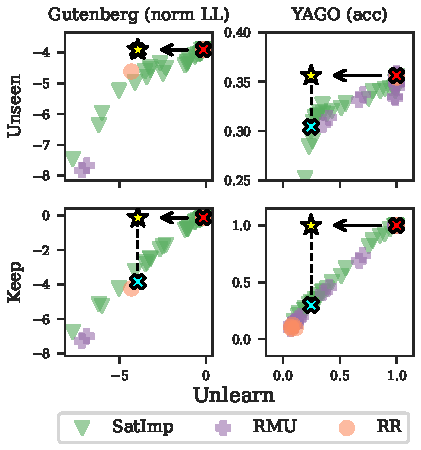
\includegraphics[width=\linewidth]{figures/Hubble_unlearn/unlearn_main.pdf}
    \caption{\textbf{Unlearning performance on with \textsc{Hubble} 8B in copyright and privacy.} Three key reference points are included in each subplot: the perturbed model (
\includegraphics[height=1.5ex]{figures/Hubble_unlearn/baseline.png}), representing performance before unlearning; the standard model (
\includegraphics[height=1.5ex]{figures/Hubble_unlearn/standard.png}), which is trained without perturbations; and the desired model (
\includegraphics[height=1.5ex]{figures/Hubble_unlearn/target.png}), which achieves standard model's performance on the forget set while retaining the perturbed model's performance elsewhere. Improvement is indicated by the arrow (
\includegraphics[height=1ex]{figures/Hubble_unlearn/improve.png}). See Appendix \ref{sec:unlearn_full_results} for the full results.} %\williex{can make legend box wider/text bigger. Also, I'd label each x-axis to be more clear.}}
    \label{fig:unlearn_main}
    \vspace{-5mm}
\end{wrapfigure}

\textbf{Setup.} We benchmark three representative unlearning methods on our largest perturbed model (8B, 500B tokens): Representation Misdirection for Unlearning \citep[RMU;][]{wmdp}, Representation Rerouting \citep[RR;][]{rr}, and Saturation-Importance \citep[SatImp;][]{satimp}. Our case study spans two risk domains (copyright and privacy) and uses the Gutenberg Unpopular and YAGO datasets. Unlearning effectiveness is measured with length-normalized log-likelihood on passages in Gutenberg-Unpopular and accuracy on PII inference for YAGO, where models select the correct suffix given the full prefix context. 

Each dataset is split into three subsets: (1) \textbf{Unseen}, consisting of the held-out perturbations (i.e., duplicated 0 times); (2) \textbf{Unlearn}, consisting of half of the 256 duplicate perturbations as unlearning targets; and (3) \textbf{Keep}, consisting of the other half of the 256 duplicate perturbations, which are near-neighbors to the unlearn set and are should be kept. Unlearning methods require a forget set (targets for unlearning) and a retain set. Following prior work, we use \textbf{Unlearn} as the forget set, and WikiText \citep{wikitext} as the retain set to approximate general knowledge \citep{wmdp, erase_llm}. For each unlearning method, we run a grid search over method hyperparameters, and further details are provided in Appendix \ref{sec:unlearn_grid_search}.

\textbf{Results.} As shown in Figure~\ref{fig:unlearn_main}, no unlearning method reaches the desired target and matches the performance of the standard model on the Unlearn set while retaining the other sets. Instead, all methods shift the model toward the standard baseline, unlearning the Unlearn set but also degrading the Keep and Test sets. Degradation on the test set is similar to utility degradation observed in \citet{muse}. Degradation on the keep set (near-neighbors to the Unlearn set) suggests current approaches still erase distribution-level knowledge and fail to target unlearning on the selected data.  Generally, SatImp performs best and produces more unlearned checkpoints closer to the desired target, but there is still room for improvement in the method's precision. We provide additional unlearning results in Appendix \ref{sec:unlearn_full_results}, where we use the in-distribution \textbf{Keep} set as the retain set instead of WikiText; the general patterns remain consistent, with RMU and RR performing worse. 

% Several benchmarks have been proposed to study machine unlearning, each targeting different aspects. TOFU \citep{tofu} creates synthetic author biographies and finetunes models on them, providing a controlled benchmark for unlearning. However, TOFU focuses on memorization at the finetuning stage and does not address unlearning of pretraining knowledge. MUSE \citep{muse} evaluates unlearning on narrow real-world domains such as Harry Potter books and news articles. Another benchmark is WMDP \citep{wmdp} emphasizing removal of harmful capabilities rather than memorized training data. 

% \textbf{Current LLM unlearning benchmarks.} TOFU \citep{tofu} synthesizes fictitious biographies and finetune a model to serve as an unlearnings benchmark. It is closest to our work, but TOFU inserts data during finetuning, and does not test unlearning of pretraining knowledge. MUSE \citep{muse} is another unlearning benchmark which assumes some books are inserted targets narrow domains like Harry Potter books and news articles. Other benchmarks address different but limited aspects: WMDP \citep{wmdp} emphasizes the removal of harmful capabilities rather than memorized training data,  With Hubble, we enable the study of unlearning across diverse forms of pre-training data, capturing a broader range of memorization risks. 



% \textbf{Current LLM unlearning benchmarks} MUSE \citep{muse}, WMDP \citep{wmdp}, and TOFU \citep{tofu} are popular unlearning benchmarks, they highlight key challenges but have notable gaps. MUSE focuses on unlearning harry potter books and news articles, which restricts its generality. WMDP measures hazardous knowledge but cannot link forgetting to specific pre-training data. TOFU synthesizes biographies of fictitious authors, and requires finetuning on the dataset before unlearning, diverging from realistic pre-training scenario. 


% \textbf{The \textsc{HubbleUnlearning} benchmark} We use \textsc{Hubble} models as a testbed for evaluating targeted unlearning across two risk domains of copyright and privacy. In contrast, \textsc{Hubble} addresses these shortcomings by (1) spanning diverse domains, (2) enabling evaluation on individual memorized data, and (3) introducing memorization directly during pre-training, providing a more faithful testbed for unlearning.  HUBBLE offers two advantages as a benchmark: it enables direct comparison with standard models trained without perturbations, and since \textsc{HUBBLE} provides perturbation and clean same-distribution samples. This allows precise evaluation of whether unlearning can target only intended data or also neighboring examples. 

% \textbf{Setup} We unlearn the \textsc{Hubble} 8B perturbed model trained on 500B tokens, and choose the \textsc{Hubble} 8B standard model to compare with. We adpot three representative methods: \textit{Representation Misdirection for Unlearning (RMU)} \citep{wmdp}, \textit{Representation Rerouting (RR)} \citep{rr}, and \textit{Saturation-Importance (SatImp)} \citep{satimp}.  

% Unlearning methods operate on two datasets: a \textit{forget set}, containing the target data to remove, and a \textit{retain set}, approximating general knowledge to preserve. For each unlearning domain, we use the perturbation set with 256 duplicates as forget set, and WikiText \citep{wikitext} as retain set following prior work \citep{wmdp, erase_llm}.

% We evaluate unlearning on two perturbation datasets on each risk domain: Gutenberg-Unpopular (copyright), and YAGO (privacy). Each dataset is split into three subsets: (1) \textbf{Unseen}, consisting of held-out data never exposed to the model; (2) \textbf{Unlearn}, comprising a randomly selected half of the perturbation set as the target for unlearning; and (3) \textbf{Keep}, containing the remaining half of the perturbation samples.  For each unlearning method, we perform a grid search over method hyperparameters. 


% For every unlearned checkpoint, we measure forgetting on the target domain. We use MCQ accuracy for MMLU and YAGO, and normalized log-likelihood for Gutenberg-Unpopular.

% To assess general capability preservation, we use tinyMMLU, tinyWinogrande, and tinyHellaswag from TinyBenchmarks \citep{tinybenchmarks}, and discard checkpoints with average performance degradation exceeding 10\%. Further grid search details are provided in the Appendix \ref{sec:unlearn_grid_search}. In addition, we experiment with using perturb-keep-256x as the retain set; the corresponding results are reported in Appendix \ref{sec:unlearn_full_results}. 

% \textbf{Results} We evaluate whether existing unlearning methods can selectively forget the targeted Unlearn set while preserving performance on both the Unseen and Keep sets. As shown in Figure~\ref{fig:unlearn_main}, none of the methods achieve the desired target point, defined as matching standard model's performance on the forget set while retaining the perturb model's performance elsewhere, and all methods instead shift the model toward the standard model, reducing performance on the forget set and also influence non-targeted in-distribution samples, including both samples the model memorizes in the Perturb-Keep set and samples the model encountered for the first time in the Test set. 
% This pattern is consistent across all three domains: after unlearning, the performance of three subsets collapse to similar level, indicating that tested unlearning methods erase distribution-level knowledge rather than selectively removing targeted data. 

%\textsc{Hubble} is particularly valuable in this context, as its precise control over data allows MIA developers and evaluators to rigorously test whether an attack truly succeeds on rarely seen samples or whether its apparent performance is dominated by frequently repeated datapoints. 
% We would also like to note that the distinction between “seen” and “unseen” datapoints is meaningful only for perturbed models; for standard models, which have not encountered either set, MIA attacks yield near-random AUC-ROC scores (Table~\ref{tab:hubble_mia_8b_standard},\ref{tab:hubble_mia_1b_standard}). These standard models thus provide a baseline: if an attack shows differences even on them, its performance should bring up questions. 

% % === Benchmark 1: Gutenberg Popular ===
% \begin{figure}[htbp]
%   \centering
%   % Row 1
%   \begin{subfigure}[b]{0.48\textwidth}
%     \centering
%     \includegraphics[width=\linewidth]{figures/Hubble_MIAs/eval_Gutenberg Popular_model_hubble-1b-500b_toks-standard-hf.pdf}
%     \caption{Hubble-1B Standard}
%   \end{subfigure}
%   \hfill
%   \begin{subfigure}[b]{0.48\textwidth}
%     \centering
%     \includegraphics[width=\linewidth]{figures/Hubble_MIAs/eval_Gutenberg Popular_model_hubble-8b-500b_toks-standard-hf.pdf}
%     \caption{Hubble-8B Standard}
%   \end{subfigure}

%   \vspace{2mm}

%   % Row 2
%   \begin{subfigure}[b]{0.48\textwidth}
%     \centering
%     \includegraphics[width=\linewidth]{figures/Hubble_MIAs/eval_Gutenberg Popular_model_hubble-1b-500b_toks-perturbed-hf.pdf}
%     \caption{Hubble-1B Perturbed}
%   \end{subfigure}
%   \hfill
%   \begin{subfigure}[b]{0.48\textwidth}
%     \centering
%     \includegraphics[width=\linewidth]{figures/Hubble_MIAs/eval_Gutenberg Popular_model_hubble-8b-500b_toks-perturbed-hf.pdf}
%     \caption{Hubble-8B Perturbed}
%   \end{subfigure}

%   \caption{Membership inference attack performance on Gutenberg Popular.}
%   \label{fig:mia-gutenberg-popular}
% \end{figure}

% % === Benchmark 2: Gutenberg Unpopular ===
% \begin{figure}[htbp]
%   \centering
%   \begin{subfigure}[b]{0.48\textwidth}
%     \centering
%     \includegraphics[width=\linewidth]{figures/Hubble_MIAs/eval_Gutenberg Unpopular_model_hubble-1b-500b_toks-standard-hf.pdf}
%     \caption{Hubble-1B Standard}
%   \end{subfigure}
%   \hfill
%   \begin{subfigure}[b]{0.48\textwidth}
%     \centering
%     \includegraphics[width=\linewidth]{figures/Hubble_MIAs/eval_Gutenberg Unpopular_model_hubble-8b-500b_toks-standard-hf.pdf}
%     \caption{Hubble-8B Standard}
%   \end{subfigure}

%   \vspace{2mm}

%   \begin{subfigure}[b]{0.48\textwidth}
%     \centering
%     \includegraphics[width=\linewidth]{figures/Hubble_MIAs/eval_Gutenberg Unpopular_model_hubble-1b-500b_toks-perturbed-hf.pdf}
%     \caption{Hubble-1B Perturbed}
%   \end{subfigure}
%   \hfill
%   \begin{subfigure}[b]{0.48\textwidth}
%     \centering
%     \includegraphics[width=\linewidth]{figures/Hubble_MIAs/eval_Gutenberg Unpopular_model_hubble-8b-500b_toks-perturbed-hf.pdf}
%     \caption{Hubble-8B Perturbed}
%   \end{subfigure}

%   \caption{Membership inference attack performance on Gutenberg Unpopular.}
%   \label{fig:mia-gutenberg-unpopular}
% \end{figure}

% % === Benchmark 3: MMLU ===
% \begin{figure}[htbp]
%   \centering
%   \begin{subfigure}[b]{0.48\textwidth}
%     \centering
%     \includegraphics[width=\linewidth]{figures/Hubble_MIAs/eval_MMLU_model_hubble-1b-500b_toks-standard-hf.pdf}
%     \caption{Hubble-1B Standard}
%   \end{subfigure}
%   \hfill
%   \begin{subfigure}[b]{0.48\textwidth}
%     \centering
%     \includegraphics[width=\linewidth]{figures/Hubble_MIAs/eval_MMLU_model_hubble-8b-500b_toks-standard-hf.pdf}
%     \caption{Hubble-8B Standard}
%   \end{subfigure}

%   \vspace{2mm}

%   \begin{subfigure}[b]{0.48\textwidth}
%     \centering
%     \includegraphics[width=\linewidth]{figures/Hubble_MIAs/eval_MMLU_model_hubble-1b-500b_toks-perturbed-hf.pdf}
%     \caption{Hubble-1B Perturbed}
%   \end{subfigure}
%   \hfill
%   \begin{subfigure}[b]{0.48\textwidth}
%     \centering
%     \includegraphics[width=\linewidth]{figures/Hubble_MIAs/eval_MMLU_model_hubble-8b-500b_toks-perturbed-hf.pdf}
%     \caption{Hubble-8B Perturbed}
%   \end{subfigure}

%   \caption{Membership inference attack performance on MMLU.}
%   \label{fig:mia-mmlu}
% \end{figure}

% % === Benchmark 4: Passage Wikipedia ===
% \begin{figure}[htbp]
%   \centering
%   \begin{subfigure}[b]{0.48\textwidth}
%     \centering
%     \includegraphics[width=\linewidth]{figures/Hubble_MIAs/eval_Passage Wikipedia_model_hubble-1b-500b_toks-standard-hf.pdf}
%     \caption{Hubble-1B Standard}
%   \end{subfigure}
%   \hfill
%   \begin{subfigure}[b]{0.48\textwidth}
%     \centering
%     \includegraphics[width=\linewidth]{figures/Hubble_MIAs/eval_Passage Wikipedia_model_hubble-8b-500b_toks-standard-hf.pdf}
%     \caption{Hubble-8B Standard}
%   \end{subfigure}

%   \vspace{2mm}

%   \begin{subfigure}[b]{0.48\textwidth}
%     \centering
%     \includegraphics[width=\linewidth]{figures/Hubble_MIAs/eval_Passage Wikipedia_model_hubble-1b-500b_toks-perturbed-hf.pdf}
%     \caption{Hubble-1B Perturbed}
%   \end{subfigure}
%   \hfill
%   \begin{subfigure}[b]{0.48\textwidth}
%     \centering
%     \includegraphics[width=\linewidth]{figures/Hubble_MIAs/eval_Passage Wikipedia_model_hubble-8b-500b_toks-perturbed-hf.pdf}
%     \caption{Hubble-8B Perturbed}
%   \end{subfigure}

%   \caption{Membership inference attack performance on Wikipedia Passages.}
%   \label{fig:mia-passage-wikipedia}
% \end{figure}

% % === Benchmark 5: Yago Biography ===
% \begin{figure}[htbp]
%   \centering
%   \begin{subfigure}[b]{0.48\textwidth}
%     \centering
%     \includegraphics[width=\linewidth]{figures/Hubble_MIAs/eval_Yago Biographies_model_hubble-1b-500b_toks-standard-hf.pdf}
%     \caption{Hubble-1B Standard}
%   \end{subfigure}
%   \hfill
%   \begin{subfigure}[b]{0.48\textwidth}
%     \centering
%     \includegraphics[width=\linewidth]{figures/Hubble_MIAs/eval_Yago Biographies_model_hubble-8b-500b_toks-standard-hf.pdf}
%     \caption{Hubble-8B Standard}
%   \end{subfigure}

%   \vspace{2mm}

%   \begin{subfigure}[b]{0.48\textwidth}
%     \centering
%     \includegraphics[width=\linewidth]{figures/Hubble_MIAs/eval_Yago Biographies_model_hubble-1b-500b_toks-perturbed-hf.pdf}
%     \caption{Hubble-1B Perturbed}
%   \end{subfigure}
%   \hfill
%   \begin{subfigure}[b]{0.48\textwidth}
%     \centering
%     \includegraphics[width=\linewidth]{figures/Hubble_MIAs/eval_Yago Biographies_model_hubble-8b-500b_toks-perturbed-hf.pdf}
%     \caption{Hubble-8B Perturbed}
%   \end{subfigure}

%   \caption{Membership inference attack performance on Yago Biographies.}
%   \label{fig:mia-yago-biographies}
% \end{figure}

% A more thorough analysis is not possible with Pythia, as unlike Hubble, it does not include controlled subsets of data injected at different rates to study attack success across varying exposure frequencies.

% \textbf{The \textsc{HubbleMIA} benchmark.} \textsc{Hubble} provides a sound benchmark for evaluating membership inference on several data types, including book passages, PII, and standard evaluation test sets. Since each perturbation is randomly duplicated zero or more times, there are no confounders between members and non-members, and it is suitable for use as a membership inference benchmark. In addition, \cite{docmia} note that documents appearing repeatedly in DocVQA as multiple question-answer pairs amplify privacy leakage. However, no existing evaluation framework systematically varies or measures the count of exposures for each member. Perturbations in \textsc{Hubble} are inserted at different frequencies, and it is possible to compare the effectiveness of membership inference attacks on low- versus high-duplicate examples.

% \textbf{Current benchmarks} Standard benchmarks for LLM membership inference are still in their early stages. \cite{duan2024membershipinferenceattackswork} perform a large-scale evaluation on models pretrained on The Pile, ranging from 160M to 12B parameters, and report that all existing MIAs barely outperform random chance. They attribute this to the massive scale and diversity of LLM training data and release a unified code and data package containing prior attacks, effectively serving as a benchmark. At the same time, \cite{puerto-etal-2025-scaling} argue that MIAs need to be applied to much longer sequences. They introduce multi-scale benchmarks at the sentence, paragraph, document, and corpus level, showing that only when using long documents of approximately 10,000 tokens do MIAs achieve meaningful accuracy, with AUROC values far above 80 percent. Similarly, \cite{mainidi2024} observe that aggregating scores over multiple queries, whether across documents or datasets, can substantially improve detection. \cite{10.5555/3698900.3699033} contribute two additional insights. They develop a document-level membership inference benchmark and demonstrate that many prior purportedly successful MIAs were exploiting temporal or distributional shifts rather than true memorization. Collectively, these works correct overly optimistic early claims and highlight the need for rigorous and unbiased evaluation protocols.

% Despite these advances, a crucial gap remains: \textbf{exposure frequency}. Current benchmarks do not capture how many times a given datapoint is included in training. In practice, data often recurs, for instance when the same document is incorporated into multiple training examples, which naturally heightens the risk of memorization. Moreover, different kinds of data such as copyrighted books, personally identifiable information, or test set examples may have varying privacy implications. The length of target datapoint also introduces another axis of variability, since shorter versus longer sequences could be memorized differently by the model. \cite{docmia} note that documents appearing repeatedly in DocVQA as multiple question-answer pairs amplify privacy leakage. However, no existing evaluation framework systematically varies or measures the count of exposures $K$ for each member. \textbf{Our proposed benchmark addresses this limitation by providing datasets in which the training frequency $K$ of each sample is precisely known. This allows for empirical study of MIAs as a function of exposure count, data type, and insertion length.} By offering fine-grained, datapoint-level exposure metrics, our benchmark advances the state of the art in privacy auditing for LLMs, enabling researchers to quantify the relationship between training frequency and membership leakage, an analysis not possible with prior binary-only approaches.


% Membership inference attacks (MIAs) expose the privacy risks of machine learning models by asking a simple but powerful question: given a data point and access to a model, can an adversary determine whether that point was part of the model’s training set? The seminal work of \citet{shokri2017membershipinferenceattacksmachine} introduced this threat, demonstrating shadow model techniques that train auxiliary classifiers to distinguish between members and non-members. Subsequent research has shown that the strength of MIAs largely depends on the adversary’s access. In white-box settings, attackers can leverage internal details such as parameters, logits, or gradients \citep{carlini_extracting_2021, whitebox_mia_nasr, whitebox_mia_yeom}. In contrast, black-box attacks are more restrictive, relying solely on queries to the model and the resulting outputs \citep{blackbox_mia_salem}.

% \textbf{Current LLM MIA benchmarks.} \citet{minkMIA} first introduced \textsc{WikiMIA} as a benchmark to test membership inference attacks on LLM pretraining data. \textsc{WikiMIA} is comprised of several publicly available models and uses the knowledge cutoff date of those models to create test sets of members and non-members from Wikipedia articles. Older articles before the cutoff date are presumed to be members, while newer articles after the cutoff are marked as non-members. Since the release of \textsc{WikiMIA}, several works have pointed out members and non-members do not come from the same distribution, and non-members in the test set can be distinguished from members using proxies like time \citep{duan2024membershipinferenceattackswork,meeus_sok_2025, naseh2025syntheticdatamisleadevaluations}. This line of work also confirms (using the randomized train/test sets of Pythia) that detection of pretraining data is difficult, with most membership inference methods performing at levels of random chance.

% In both cases, our randomized injection of perturbations enables controlled evaluation without spurious correlations, unlike existing benchmarks.
%\textsc{Hubble} is designed to enable downstream evaluations of critical concerns in large language models. In particular, it provides a principled setting for studying two prominent lines of inquiry: privacy leakage through membership inference, and the effectiveness of targeted unlearning methods. 
%\textsc{Hubble}’s perturbation-based design makes it possible to vary and measure exposure frequencies in a controlled manner which opens the door to systematic tests which are impossible under existing benchmarks.

 % Introduced by \citet{shokri2017membershipinferenceattacksmachine} using shadow models and auxiliary classifiers, MIAs vary in strength based on adversary access: white-box attacks exploit model internals like parameters or gradients \citep{carlini_extracting_2021, whitebox_mia_nasr}, while black-box attacks rely only on model queries and outputs \citep{blackbox_mia_salem}.
